
\section{区分辛结构}\label{sec:9-7}
\zhindex{qufenxinjiegou}{区分辛结构}

本章最后讨论用 $J$-全纯球面区分\BookRecordIndex{T0358}辛流形的若干情形。这样的例子比人们可能预期的要少。
一个困难在于\BookRecordIndex{T0143}格罗莫夫--威滕不变量不易计算。（有了辛和公式以后，这件事容易了一些；
见 Ionel--Parker \srcite{200,201} 与 Li--Ruan \srcite{238}。）更根本的问题是，球面的
行为往往与所研究的问题无关。

一个基本事实是，在四维情形，Taubes \srcite{390,391,392,393} 和 Ionel--Parker
\srcite{198} 的工作说明，最初等的\BookRecordIndex{T0143}格罗莫夫--威滕不变量（即计数通过适当数目点的、
任意亏格的嵌入 \BookRecordIndex{T0003}$J$-全纯曲线的那些不变量）与 Seiberg--Witten 不变量包含相同信息，
因而只依赖于 $M$ 的光滑结构。因此在四维中，我们不能用\BookRecordIndex{T0143}格罗莫夫--威滕不变量区分同一
光滑流形上的不同辛结构。此外，尽管同胚四维流形在与 $S^2$ 作乘积后会成为微分同胚的，
下面的例~\ref{ex:9-7-1} 将说明，\BookRecordIndex{T0143}格罗莫夫--威滕不变量的差异在这一操作下仍然存在。这与
Donaldson 关于 Lefschetz 铅笔的工作 \srcite{85} 一起表明：与光滑情形不同，\BookRecordIndex{T0358}辛流形
的拓扑并不会随着维数增加而变得更容易理解。事实上，Donaldson 猜想，两个辛四维流形
$(M,\omega)$ 与 $(M',\omega')$ 微分同胚，当且仅当带乘积辛结构的六维流形
$M\times S^2$ 与 $M'\times S^2$ 形变等价。（值得注意的是，Smith 在 \srcite{382}
中构造了一些例子，说明若把二维球面换成第一 Chern 类可被某个整数 $N>2$ 整除的任意
\BookRecordIndex{T0358}辛流形，例如二维环面或 $\mathbb CP^2$，则这个猜想的“仅当”部分不成立。）

因此，近期许多理解\BookRecordIndex{T0358}辛流形结构的工作都集中在四维情形，\footnote{六维中也开始出现一些
有趣的新构造；见 Fine--Panov \srcite{109}。}并被纳入理解光滑流形这一更大的问题中。
人们投入了大量精力构造有趣的例子。这个方向的早期工作见 Gompf \srcite{154}、
Fintushel--Stern \srcite{110}、Szabo \srcite{387} 及其中的参考文献。较近以来，
人们多次尝试在与 $\mathbb CP^2$ 的 $k$ 点吹起同胚的流形上寻找奇异光滑结构或辛结构。
在本书写作时，存在这种结构的最小 $k$ 值仍然未知，当前纪录是 $k=2$；见
Akhmedov--Park \srcite{10}、Baldridge--Kirk \srcite{30} 与 Fintushel--Stern
\srcite{111}。另一项重要任务称为\emph{\BookRecordIndex{T0100}地理问题}：给定基本群，研究辛四维流形
$(M,\omega)$ 上 $\omega$-\BookRecordIndex{T0372}驯服\BookRecordIndex{T0088}殆复结构的示性数所给出的传统不变量之取值范围。

无论如何，本书所讨论的亏格零\BookRecordIndex{T0143}格罗莫夫--威滕不变量并未给这些问题带来新信息，因为
Li--Liu \srcite{240} 证明了，它们只在有理流形和直纹流形的吹起（带标准光滑结构）上
非零。迄今为止，用来探测给定光滑四维流形 $X$ 上不同\BookRecordIndex{T0363}辛形式的唯一不变量，是相应被\BookRecordIndex{T0372}驯服
\BookRecordIndex{T0088}殆复结构的 Chern 类；见注~\ref{rem:9-4-3}(iv)。Donaldson--Smith 的论文 \srcite{89} 所开启的
发展，或许会使高亏格 \BookRecordIndex{T0003}$J$-全纯曲线在理解辛四维流形时更有用。探测辛四维流形之间更细微
差异的一种可能方法，是像 Auroux--Katzarkov \srcite{28} 的工作那样，把它们看成
$\mathbb CP^2$ 的分支覆叠；也见 Auroux 的综述 \srcite{27}。

本节只介绍两个例子，二者都在六维。通过与若干个 $S^2$ 作乘积，它们可以推广到更高
维数。我们先概述 Ruan 的一项工作；它无疑影响了 Donaldson 提出上述猜想。然后介绍
McDuff 的一项工作，其中构造了两个上同调的\BookRecordIndex{T0363}辛形式：它们能由形变相连，却不能由同痕
相连。这里使用的不变量取自\BookRecordIndex{T0283}求值映射所携带的同伦信息，而不是同调信息。关于利用 \BookRecordIndex{T0021}Fukaya
范畴性质研究这个问题的一种全新方法，见 Seidel \srcite{373}。

\begin{example}[非形变等价的六维流形]\label{ex:9-7-1}
这个例子源于 Ruan \srcite{340}，并且只是许多例子中的一个。设 $X$ 是
$\mathbb CP^2$ 在 $8$ 个点处的吹起，$Y$ 是 Barlow 曲面。这两个流形都是单连通的，
而且具有相同的相交形式，所以它们同胚，但并不微分同胚。由 Wall 的结果，稳定化流形
\[
  X':=X\times S^2,\qquad Y':=Y\times S^2
\]
微分同胚。此外，二者都是 \BookRecordIndex{T0207}凯勒 流形，并且可以选取微分同胚
\[
  \psi:X'\longrightarrow Y'
\]
使它保持各自复结构的 Chern 类。后一陈述意味着，$\psi$ 把 $X'$ 上的乘积复结构 $J_X$
送到与 $Y'$ 上乘积复结构 $J_Y$ 同伦的结构 $\psi_*J_X$。此外，利用杯积的一个简单论证
可得 $\psi_*[X\times\mathrm{pt}]=[Y\times\mathrm{pt}]$。由此可说明，同态
\[
  \psi_*:H_2(X')\longrightarrow H_2(Y')
\]
把子集 $H_2(X)\subset H_2(X')$ 与 $H_2(Y)\subset H_2(Y')$ 等同起来，而且所得同构
$H_2(X)\to H_2(Y)$ 保持相交形式。

在任意 \BookRecordIndex{T0207}凯勒 流形上，凯勒 形式之集都是凸锥，所以任意两个这样的形式都可以由一个
形变相连。因此，\BookRecordIndex{T0207}凯勒 流形 $X',Y'$ 带有在形变意义下唯一确定的\BookRecordIndex{T0363}辛形式
$\omega_{X'},\omega_{Y'}$；自然要问，偶对 $(X',\omega_{X'})$ 与
$(Y',\omega_{Y'})$ 是否形变等价。Ruan 通过证明\BookRecordIndex{T0143}格罗莫夫--威滕不变量
\[
  \operatorname{GW}_{E',1}^{X'}(\operatorname{PD}(E'))=-1
\]
说明答案是否定的。这里 $E'\in H_2(X';\mathbb Z)$ 是 $X$ 中一个吹起点的类
$E\in H_2(X;\mathbb Z)$ 在同态
$H_2(X;\mathbb Z)\to H_2(X';\mathbb Z)$ 下的像；而对
$F':=\psi_*E'$，相应的不变量为零：
\[
  \operatorname{GW}_{F',1}^{Y'}(\operatorname{PD}(F'))=0.
\]
\BookRecordIndex{T0143}格罗莫夫--威滕不变量在形变等价下不变，所以这说明
$(X',\omega_{X'})$ 与 $(Y',\omega_{Y'})$ 不等价。

还须计算这两个\BookRecordIndex{T0143}格罗莫夫--威滕不变量。因为 $c_1(E')=1$ 且
$\dim X'=2n=6$，有
\[
  \dim\mathcal M_{0,1}(E')
  =2n+2c_1(E')+2-6=4=2n-\deg(E'),
\]
所以定义 $\operatorname{GW}_{E',1}^{X'}(\operatorname{PD}(E'))$ 所需的维数条件成立。
此外，$X$ 中恰有一个表示 $E$ 的全纯球面 $C$。因此，
$X'=X\times S^2$ 中的 $E'$-曲线恰是 $z\in S^2$ 时的曲线
$C\times\{z\}$。故\BookRecordIndex{T0283}求值映射
\[
  \operatorname{ev}:\mathcal M_{0,1}(E';J_X)\longrightarrow X'
\]
的像是子流形 $C\times S^2\subset X'$。于是
$\operatorname{ev}\mathbin{\boldsymbol\cdot}E'=-1$，从而
\[
  \operatorname{GW}_{E',1}^{X'}(\operatorname{PD}(E'))=-1.
\]

另一方面，Barlow 曲面 $Y$ 是极小的，所以不存在自交数为 $-1$ 的嵌入全纯球面。又由
上面的讨论，同调类
\[
  F':=\psi_*E'\in H_2(Y')
\]
是某个自交数 $F\mathbin{\boldsymbol\cdot}F=-1$ 的类 $F\in H_2(Y)$ 在同态
$H_2(Y)\to H_2(Y')$ 下的像。由于 $J_Y$ 与 $\psi_*J_X$ 同伦，有 $c_1(F)=1$。
现在固定 $Y$ 上一个与 $\omega_Y$ \BookRecordIndex{T0348}相容的\BookRecordIndex{T0088}殆复结构，使每个全纯球面都有正 Chern 数，
并仍以 $J_Y$ 表示 $Y'=Y\times S^2$ 上相应的乘积结构。我们断言，不存在表示 $F'$ 的
亏格零 $J_Y$-全纯\BookRecordIndex{T0340}稳定映射。事实上，对这样的\BookRecordIndex{T0340}稳定映射的每个分支，与投影
$Y'\to S^2$ 的复合都有非负次数。$F'$ 在诱导同态
$H_2(Y')\to H_2(S^2)$ 下的像为零，故\BookRecordIndex{T0340}稳定映射的每个分支都投影到 $S^2$ 中的一点。
因此，$Y$ 中必须存在表示 $F$ 的\BookRecordIndex{T0340}稳定映射。这样一张\BookRecordIndex{T0340}稳定映射的每个分支都有正 Chern
数，所以它只能有一个 Chern 数为一且自交数为负一的分支。由\BookRecordIndex{T0054}伴随不等式，这样的全纯
球面必为嵌入，这与 $Y$ 的极小性矛盾。因此 $F'$ 不能由 $J_Y$-全纯\BookRecordIndex{T0340}稳定映射表示，
从而\BookRecordIndex{T0363}辛形式 $\omega_{Y'}$ 的\BookRecordIndex{T0143}格罗莫夫--威滕不变量
$\operatorname{GW}_{F',1}^{Y'}$ 为零。
\end{example}

第二个例子建立在 $S^2\times S^2$ 的如下微分同胚环路的性质之上：对
$t\in\mathbb R/\mathbb Z$，定义
$\psi_t:S^2\times S^2\to S^2\times S^2$ 为
\begin{equation}\label{eq:9-7-1}
  \psi_t(z,w)=(z,\Phi_{z,t}(w)),
\end{equation}
其中 $\Phi_{z,t}$ 表示把单位球面 $S^2\subset\mathbb R^3$ 绕通过 $z,-z$ 的轴旋转
角度 $2\pi t$。因此，$\psi_t$ 固定 $S^2\times S^2$ 的对角线
$\{(z,z)\mid z\in S^2\}$ 上的所有点，也固定反对角线
$\{(z,-z)\mid z\in S^2\}$ 上的所有点。

以 $\sigma$ 表示 $S^2$ 上总面积为 $4\pi$ 的标准面积形式，并考虑
$S^2\times S^2$ 上的\BookRecordIndex{T0363}辛形式族
\[
  \omega_\lambda:=\lambda\pi_1^*\sigma+\pi_2^*\sigma,
  \qquad \lambda\ge1.
\]
这里把第一个球面选成较大的那个；我们把它看成纤维丛
$\pi_1:S^2\times S^2\to S^2$ 的底。令 $\mathcal H$ 表示从
$S^2\times S^2$ 到自身、并在同调上诱导恒等映射的连续映射之空间。

\begin{proposition}\label{prop:9-7-2}
\begin{enumerate}[label=\textnormal{(\roman*)}]
\item 环路 $\{\psi_t\}$ 在 $\pi_1(\mathcal H,\operatorname{id})$ 中具有无穷阶。
\item 环路 $\{\psi_t\}$ 同痕于
$\operatorname{Ham}(S^2\times S^2,\omega_\lambda)$ 中的一条环路，当且仅当
$\lambda>1$。
\end{enumerate}
\end{proposition}

注意，(ii) 中的“仅当”部分立即由 (i) 以及
$\operatorname{Ham}(S^2\times S^2,\omega_1)$ 与
$\operatorname{SO}(3)\times\operatorname{SO}(3)$ 同伦等价这一事实\BookRecordIndex{T0326}推出（见定理
~\ref{thm:9-5-1}）。这意味着
$\pi_1(\operatorname{Ham}(S^2\times S^2,\omega_1))$ 是有限群，因而不可能包含
一个在更大空间中具有无穷阶的元素 $\{\psi_t\}$。实际上，当 $0<\lambda<1$ 时，
$\{\psi_t\}$ 也不能同伦到 $\operatorname{Ham}(S^2\times S^2,\omega_\lambda)$
中，但这需要进一步的论证。这里我们只考虑 $\lambda\ge1$，所以无须讨论这种情形。
(ii) 中“如果”部分的证明推迟到本节末尾。例 11.4.9 还将概述 (ii) 的另一种证明；它
使用 \BookRecordIndex{T0047}Seidel 表示的性质，而不使用定理~\ref{thm:9-4-7}。

断言 (i) 是下一个引理的直接推论；该引理也将在本节末尾证明。它基于映射
$Y\to S^2$ 的广义 Hopf 不变量之性质，其中定义域 $Y$ 是紧定向光滑三维流形，而且映射
诱导零同态 $H_2(Y)\to H_2(S^2)$。为简便起见，我们称这样的映射在 $H_2$ 上为零。

\begin{lemma}\label{lem:9-7-3}
固定一点 $w_0\in S^2$。对 $k\in\mathbb Z$，定义
$F^k:S^1\times S^2\to S^2$ 为
\[
  F^k(t,z):=\Phi_{z,kt}(w_0).
\]
则 $F^k$ 与 $F^\ell$ 能够通过一个在 $H_2$ 上为零的映射配边，当且仅当 $k=\ell$。
\end{lemma}

\begin{proof}[命题~\ref{prop:9-7-2}(i) 的证明]
每个环路 $\mathbb R/\mathbb Z\to\mathcal H:t\mapsto\psi_t$ 都通过
\[
  F_\psi(t,z):=\pi_2(\psi_t(z,w_0))
\]
决定连续映射 $F_\psi:S^1\times S^2\to S^2$，其中
$\pi_2:S^2\times S^2\to S^2$ 是到第二个因子的投影。若两个环路 $\psi,\psi'$ 同伦，
则相应的映射 $F_\psi,F_{\psi'}$ 也同伦。进一步，由于 $F_\psi,F_{\psi'}$ 本身在
$H_2$ 上为零，连接它们的任意同伦在 $H_2$ 上也为零。令
$\psi^k=\{\psi_t^k\}$ 表示环路 $t\mapsto\psi_{kt}$，其中 $\psi_t$ 由式
~\eqref{eq:9-7-1} 定义。于是 $F_{\psi^k}=F^k$。由引理~\ref{lem:9-7-3}，
$\psi^k$ 与 $\psi^\ell$ 同伦当且仅当 $k=\ell$。这证明了命题
~\ref{prop:9-7-2}(i)。
\end{proof}

考虑 $X:=S^2\times S^2\times\mathbb T^2$ 上的如下两族形式。第一族是乘积形式
\[
  \tau_\lambda^0:=\lambda\pi_1^*\sigma+\pi_2^*\sigma+ds\wedge dt,
\]
第二族是 $\tau_\lambda^1:=\Psi_*\tau_\lambda^0$，其中微分同胚
$\Psi:X\to X$ 定义为
\[
  \Psi(z,w,s,t)=(z,\Phi_{z,t}(w),s,t),
\]
而形式上的推前 $\Psi_*$ 定义为 $(\Psi^{-1})^*$。

\begin{theorem}\label{thm:9-7-4}
当 $\lambda>1$ 时，$S^2\times S^2\times\mathbb T^2$ 上的\BookRecordIndex{T0363}辛形式
$\tau_\lambda^0$ 与 $\tau_\lambda^1$ 同痕。当 $\lambda=1$ 时，它们上同调，并且可以
由一条\BookRecordIndex{T0363}辛形式道路相连，但并不同痕。
\end{theorem}

\begin{proof}
当 $\lambda>1$ 时，两形式同痕是命题~\ref{prop:9-7-2} 的推论。事实上，此时 $\Psi$
同痕于形如
\[
  (z,w,s,t)\longmapsto(\psi_t'(z,w),s,t)
\]
的微分同胚 $\Psi'$，其中 $(\psi_t')^*\omega_\lambda=\omega_\lambda$。所以
$\Psi'_*\tau_\lambda^0$ 形如
$\tau_\lambda^0+dt\wedge\pi^*\alpha_t$，其中 $\alpha_t$ 是
$S^2\times S^2$ 上一族光滑的正合 $1$-形式，而
$\pi:X\to S^2\times S^2$ 是显然的投影。因此，线性道路
\[
  \mu\Psi'_*\tau_\lambda^0+(1-\mu)\tau_\lambda^0
\]
由彼此上同调的\BookRecordIndex{T0363}辛形式组成。现在应用 Moser 同痕（见注~\ref{rem:9-4-9}）。

由此也可知，\BookRecordIndex{T0363}辛形式 $\tau_1^0$ 与 $\tau_1^1$ 能由一条\BookRecordIndex{T0363}辛形式道路相连。它们因而定义相同
的 Chern 类，而且显然彼此上同调。所以，这对形式的“经典不变量”相同。

为了说明 $\tau_1^0$ 与 $\tau_1^1$ 并不同痕，考察类
\[
  A:=[S^2\times\mathrm{pt}\times\mathrm{pt}]
\]
中球面的\BookRecordIndex{T0246}模空间 $\mathcal M(A;J)$。由于 $\lambda=1$，$A$ 是不\BookRecordIndex{T0213}可分解类。因此，对每个
$J\in\mathcal J(X,\tau_1^0)$，$\mathcal M(A;J)/G$ 都紧。若 $J$ 对 $A$ 正则且与
$\tau_1^0$ \BookRecordIndex{T0348}相容，则 $\mathcal M(A;J)/G$ 是紧光滑四维流形。显然的乘积结构 $J^0$
对 $A$ 正则并与 $\tau_1^0$ \BookRecordIndex{T0348}相容。\BookRecordIndex{T0246}模空间 $\mathcal M(A;J^0)/G$ 可通过微分同胚
\[
  S^2\times\mathbb T^2\longrightarrow\mathcal M(A;J^0)/G,
  \qquad (w,s,t)\longmapsto[u_{w,s,t}],
  \qquad u_{w,s,t}(z):=(z,w,s,t)
\]
与 $S^2\times\mathbb T^2$ 等同。再考虑与 $\tau_1^1$ \BookRecordIndex{T0348}相容的\BookRecordIndex{T0088}殆复结构
$J^1:=\Psi_*J^0$。它与 $J^0$ 微分同胚，因而也对 $A$ 正则。
$\mathcal M(A;J^1)$ 的元素是等价类 $[\Psi\circ u_{w,s,t}]$。

反设\BookRecordIndex{T0363}辛形式 $\tau_1^0,\tau_1^1$ 通过一族光滑的彼此上同调的\BookRecordIndex{T0363}辛形式
$\tau_1^r$（$0\le r\le1$）同痕。于是存在一族正则\BookRecordIndex{T0088}殆复结构
$J^r\in\mathcal J(X,\tau_1^r)$（$0\le r\le1$），使相应的\BookRecordIndex{T0246}模空间
\[
  \mathcal W(A;\{J^r\})
  :=\{(r,u)\mid0\le r\le1,\ u\in\mathcal M(A;J^r)\}
\]
给出从 $\mathcal M(A;J^0)/G$ 到 $\mathcal M(A;J^1)/G$ 的紧\BookRecordIndex{T0107}定向配边
$\mathcal W(A;\{J^r\})/G$。相应的\BookRecordIndex{T0283}求值映射
\[
  \operatorname{ev}:\mathcal W(A;\{J^r\})\times_GS^2
  \longrightarrow[0,1]\times X,
  \qquad \operatorname{ev}([r,u,z]):=(r,u(z))
\]
是两个带边紧定向七维流形之间的光滑映射。考虑嵌入圆周
$\gamma^0,\gamma^1\subset X$：
\[
  \gamma^0:=\{(z_0,w_0,s_0,t)\mid t\in S^1\},
  \qquad
  \gamma^1:=\{(z_0,\Phi_{z_0,t}(w_0),s_0,t)\mid t\in S^1\}
  =\Psi(\gamma^0).
\]
这两个子流形都微分同胚于圆周，并且\BookRecordIndex{T0107}定向配边；也就是说，存在定向二维流形
$\sigma\subset[0,1]\times X$，其边界为
\[
  \partial\sigma
  =\sigma\cap(\{0,1\}\times X)
  =(\{0\}\times\gamma^0)\cup(\{1\}\times\gamma^1).
\]
注意，$\operatorname{ev}$ 在
$\mathcal W(A;\{J^r\})\times_GS^2$ 的边界上的限制与 $\partial\sigma$ 横截。必要时在
$[0,1]\times X$ 的内部扰动 $\sigma$，还可假设 $\operatorname{ev}$ 与 $\sigma$
横截。于是
$\Sigma:=\operatorname{ev}^{-1}(\sigma)$ 是带边紧定向光滑二维流形。它由
\[
  \Sigma=\mathcal W(A,\sigma;\{J^r\})/G
\]
给出，其中
\[
  \mathcal W(A,\sigma;\{J^r\})
  :=\bigl\{(r,u,z)\bigm|0\le r\le1,\ u\in\mathcal M(A;J^r),\ z\in S^2,
  \ (r,u(z))\in\sigma\bigr\},
\]
而其边界是
$\partial\Sigma=(\{0\}\times\Gamma^0)\cup(\{1\}\times\Gamma^1)$。这里
$\Gamma^0\subset\mathcal M(A;J^0)\times_GS^2$ 与
$\Gamma^1\subset\mathcal M(A;J^1)\times_GS^2$ 是嵌入圆周
\[
  \Gamma^0:=\{[u_{w_0,s_0,t},z_0]\mid t\in S^1\},
  \qquad
  \Gamma^1:=\{[\Psi\circ u_{w_0,s_0,t},z_0]\mid t\in S^1\}.
\]

现在考虑\BookRecordIndex{T0246}模空间
\[
  W:=\mathcal W(A,\sigma;\{J^r\})\times_GS^2,
\]
其边界为 $\partial W=(\{0\}\times Y^0)\cup(\{1\}\times Y^1)$，其中
$Y^0,Y^1$ 都微分同胚于 $S^1\times S^2$。\BookRecordIndex{T0246}模空间 $W$ 带有纤维为 $S^2$ 的投影
$\pi:W\to\Sigma$，以及\BookRecordIndex{T0283}求值映射 $F:W\to S^2$；后者由
$F([r,u,z,z']):=\pi_2(u(z'))$ 给出，其中
$\pi_2:S^2\times S^2\times\mathbb T^2\to S^2$ 是到第二个因子的投影：
\[
\begin{tikzpicture}[baseline=(current bounding box.center),>=stealth]
  \node (w) at (0,0) {$W$};
  \node (s2) at (3.2,0) {$S^2$};
  \node (sig) at (0,-1.25) {$\Sigma$};
  \draw[->] (w) -- node[above] {$F$} (s2);
  \draw[->] (w) -- node[left] {$\pi$} (sig);
\end{tikzpicture}
\]
在与 $S^1\times S^2$ 的等同下，$F$ 到两个边界分支的限制分别是
\[
  F^0(t,z')=w_0,
  \qquad
  F^1(t,z')=\Phi_{z',t}(w_0).
\]
由于 $W$ 是 $\Sigma$ 上的局部平凡\BookRecordIndex{T0279}纤维化，$F$ 到 $W$ 的所有具有非空边界的连通分支
之并的限制在 $H_2$ 上为零，并给出从 $F^0$ 到 $F^1$ 的配边。这与引理
~\ref{lem:9-7-3} 矛盾，从而证明了定理~\ref{thm:9-7-4}。
\end{proof}

\begin{proof}[引理~\ref{lem:9-7-3} 的证明]
设 $Y$ 是紧定向光滑三维流形。光滑映射 $S^3\to S^2$ 的 Hopf 不变量，可以如下推广到
在 $H_2$ 上为零的光滑映射 $F:Y\to S^2$。设 $x,y$ 是 $F$ 的两个\BookRecordIndex{T0409}正则值，并用
\[
  \alpha:=F^{-1}(x),\qquad \beta:=F^{-1}(y)
\]
表示它们的原像。由于诱导映射 $F_*:H_2(Y)\to H_2(S^2)$ 为零，定向一维流形
$\alpha,\beta$ 都零同调。选取边界为 $\partial\Sigma=\alpha$ 的定向光滑链
$\Sigma\subset Y$，定义 $F$ 的 \emph{Hopf 数}为
\[
  \chi(F):=\Sigma\mathbin{\boldsymbol\cdot}\beta.
\]
若 $\Sigma'$ 是另一条这样的链，则 $\Sigma\cup(-\Sigma')$ 在 $Y$ 中定义闭链。由于
$\beta$ 零同调，它与这条闭链的相交数为零，所以 $\chi(F)$ 与 $\Sigma$ 的选取无关。
它与 $x,y$ 的选取也无关，这可由微分拓扑中的通常论证得出，参见 Milnor \srcite{289}。

现在设 $F_0:Y_0\to S^2$ 与 $F_1:Y_1\to S^2$ 能够通过一个在 $H_2$ 上为零的映射
配边。于是存在紧定向光滑四维流形 $W$ 和光滑映射 $F:W\to S^2$，使
\[
  \partial W=\overline Y_0\cup Y_1,
  \qquad F|_{Y_0}=F_0,
  \qquad F|_{Y_1}=F_1,
\]
其中 $\overline Y_0$ 表示反转 $Y_0$ 的定向。取 $x,y\in S^2$ 为
$F_0,F_1,F$ 的两个互异公共\BookRecordIndex{T0409}正则值，并记
\[
  \alpha_0:=F_0^{-1}(x),\quad
  \alpha_1:=F_1^{-1}(x),\quad
  \sigma:=F^{-1}(x),
\]
\[
  \beta_0:=F_0^{-1}(y),\quad
  \beta_1:=F_1^{-1}(y),\quad
  \tau:=F^{-1}(y).
\]
于是 $\sigma,\tau\subset W$ 是定向二维流形，其边界分别为
$\partial\sigma=\overline\alpha_0\cup\alpha_1$ 与
$\partial\tau=\overline\beta_0\cup\beta_1$。选取定向链
$\Sigma_0\subset Y_0$、$\Sigma_1\subset Y_1$，使
$\partial\Sigma_0=\alpha_0$、$\partial\Sigma_1=\alpha_1$。于是
$\Sigma:=\Sigma_0\cup\sigma\cup\overline\Sigma_1$ 是 $W$ 中的闭链，因而
\[
  \chi(F_0)-\chi(F_1)
  =\beta_0\mathbin{\boldsymbol\cdot}\Sigma_0
   +\beta_1\mathbin{\boldsymbol\cdot}\overline\Sigma_1
  =\tau\mathbin{\boldsymbol\cdot}\Sigma=0.
\]
第二个等号来自把 $\Sigma$ 扰动成 $W$ 内部的一般链，并使用
$\tau\cap\sigma=\varnothing$。最后一个等号来自如下事实：$F$ 在 $H_2$ 上为零，所以
对每个 $y\in S^2$，$F^{-1}(y)$ 在 $H_2(W,\partial W)$ 中零同调。

我们断言，对每个 $k\in\mathbb Z$ 都有 $\chi(F^k)=k$。先设 $k=1$，考虑
$F(t,z):=F^1(t,z)=\Phi_{z,t}(w_0)$。每个 $x\ne w_0$ 都是 $F$ 的\BookRecordIndex{T0409}正则值。取
$x:=-w_0$，则其原像是子流形
\[
  \alpha:=F^{-1}(-w_0)
  =\{(t,z)\mid t=1/2,\ z\perp w_0\}.
\]
这里把 $S^2$ 与 $\mathbb R^3$ 中的单位球面等同，并用 $\mathbb R^3$ 的标准内积定义
$\perp$。再任取另一个\BookRecordIndex{T0409}正则值 $y\in S^2\setminus\{\pm w_0\}$。原像
$\beta:=F^{-1}(y)$ 是所有满足如下条件的偶对 $(t,z)$ 之集：$z$ 垂直于 $y-w_0$，并且
在垂直于 $z$ 的定向平面中，从 $w_0$ 到 $y$ 的角度为 $2\pi t$。所以 $\beta$ 与
$\{1/2\}\times S^2\setminus\alpha$ 的每个半球恰好横截于一点。两个交点形如
$(1/2,z)$，其中 $z$ 垂直于 $y-w_0$，并位于通过 $w_0,y$ 的大圆上。这说明
$|\chi(F)|=1$；符号留给读者验证。

当 $k>0$ 时，不变量 $\chi(F^k)$ 的公式同理可证。具体地，
$\alpha_k:=(F^k)^{-1}(-w_0)$ 是 $k$ 个不交圆周
\[
  \bigl\{((2i-1)/2k,z)\bigm|z\perp w_0\bigr\},
  \qquad i=1,\ldots,k,
\]
之并。与上面一样，$\beta_k:=(F^k)^{-1}(y)$ 与
$\{(2i-1)/2k\}\times S^2\setminus\alpha_k$ 的每个半球恰交于一点。把 $k$ 换成
$-k$，等价于反转 $S^1\times S^2$ 的定向而保持 $F^k$ 不变。于是共有三处符号改变，
分别来自 $\alpha_k$、$\beta_k$ 与 $S^1\times S^2$ 的定向。因此
$\chi(F^{-k})=-\chi(F^k)$，引理得证。
\end{proof}

\begin{proof}[命题~\ref{prop:9-7-2}(ii) 的第一个证明]
命题陈述之后已经证明了“仅当”部分，所以只须考虑“如果”部分。下面给出两个证明：
第一个直接计算，第二个更具概念性。

注意，微分同胚 $\psi_t$ 定义了 $S^2\times S^2$ 上的光滑 $S^1$-作用。把\BookRecordIndex{T0363}辛形式
$\omega_\lambda$ 关于这个作用平均，得到闭 $2$-形式
\[
  \omega_\lambda':=\int_0^1\psi_t^*\omega_\lambda\,dt.
\]
由构造，它表示与 $\omega_\lambda$ 相同的上同调类，并且对每个 $t$ 都由 $\psi_t$
保持。直接计算（习题~\ref{ex:9-7-5}）表明
\begin{align}
&\omega'_{\lambda,(z,w)}
  \bigl((\dot z_1,\dot w_1),(\dot z_2,\dot w_2)\bigr)\notag\\
&\quad=\lambda\langle z\times\dot z_1,\dot z_2\rangle
  +\langle w\times\dot w_1,\dot w_2\rangle\notag\\
&\qquad-\langle z\times\dot z_1,\dot w_2\rangle
  +\langle z\times\dot z_2,\dot w_1\rangle
  +2\langle z,w\rangle\langle z\times\dot z_1,\dot z_2\rangle.
  \label{eq:9-7-2}
\end{align}
这里 $\times$ 表示向量积，$\langle\cdot,\cdot\rangle$ 表示 $\mathbb R^3$ 上的标准内积。
为了证明对每个 $\lambda>1$，$\omega_\lambda'$ 都非退化，须对每个
$(z,w)\in S^2\times S^2$ 及每对切向量
$\dot z_1\in T_zS^2$、$\dot w_1\in T_wS^2$ 证明：若式~\eqref{eq:9-7-2}
右边对所有 $\dot w_2,\dot z_2$ 都为零，则 $\dot w_1=\dot z_1=0$。给定这样一对切向量
$(\dot z_1,\dot w_1)$。令 $\dot z_2=0$ 并让 $\dot w_2$ 自由变化，可得
\begin{equation}\label{eq:9-7-3}
  \dot w_1+w\times(z\times\dot z_1)=0.
\end{equation}
所以对每个 $\dot z_2\in T_zS^2$ 都有
\begin{equation}\label{eq:9-7-4}
  \langle z\times\dot z_2,\dot w_1\rangle
  +\langle z,w\rangle
   \langle z\times\dot z_1,\dot z_2\rangle=0.
\end{equation}
（对 $\dot z_j\perp z$，使用公式
$(z\times\dot z_1)\times(z\times\dot z_2)
=\langle z\times\dot z_1,\dot z_2\rangle z$。）现在再令 $\dot w_2=0$，由式
~\eqref{eq:9-7-4} 得
\[
  (\lambda+\langle z,w\rangle)
  \langle z\times\dot z_1,\dot z_2\rangle=0
\]
对每个 $\dot z_2\in T_zS^2$ 都成立。因为
$|\langle z,w\rangle|\le1<\lambda$，这蕴含 $\dot z_1=0$；再由式
~\eqref{eq:9-7-3}，$\dot w_1=0$。所以 $\omega_\lambda'$ 对 $\lambda>1$ 非退化。
类似论证还说明，$2$-形式
\[
  \omega_{\lambda,s}:=\omega_\lambda+s(\omega_\lambda'-\omega_\lambda)
\]
对每个 $s\in[0,1]$ 都非退化。由 Moser 同痕（见注~\ref{rem:9-4-9}），存在与恒等映射同痕的
微分同胚 $\phi:S^2\times S^2\to S^2\times S^2$，使
$\phi^*\omega_\lambda'=\omega_\lambda$。因此，环路
$t\mapsto\phi^{-1}\circ\psi_t\circ\phi$ 与 $t\mapsto\psi_t$ 光滑同痕，并且保持\BookRecordIndex{T0363}辛
形式 $\omega_\lambda$。这就完成了命题~\ref{prop:9-7-2}(ii) 的第一个证明。
\end{proof}

\begin{exercise}\label{ex:9-7-5}
推导命题~\ref{prop:9-7-2} 的上述证明中的公式~\eqref{eq:9-7-2}。

\emph{提示：}把 $S^2$ 与 $\mathbb R^3$ 中的单位球面等同。于是，$S^2$ 上总面积为
$4\pi$ 的标准\BookRecordIndex{T0363}辛形式是
\[
  \sigma_w(\dot w_1,\dot w_2)
  =\langle w\times\dot w_1,\dot w_2\rangle,
\]
而微分同胚 $\Phi_{z,t}:S^2\to S^2$ 为
\[
  \Phi_{z,t}(w)
  =\cos(2\pi t)\bigl(w-\langle z,w\rangle z\bigr)
   +\langle z,w\rangle z+\sin(2\pi t)z\times w.
\]
给定道路 $\mathbb R\to S^2:s\mapsto z(s)$，证明 $S^2$ 的同痕
$s\mapsto\Phi_{z(s),t}$ 由向量场
\[
  X_{z,\dot z,t}(w)
  :=\bigl(\sin(2\pi t)\dot z
  +(1-\cos(2\pi t))z\times\dot z\bigr)\times w
\]
生成，其中 $z\in S^2$、$\dot z\in T_zS^2$、$t\in\mathbb R$。证明
$\Phi_{z,t}^*X_{z,\dot z,t}=-X_{z,\dot z,-t}$。再证明，在微分同胚
$\psi_t(z,w)=(z,\Phi_{z,t}(w))$ 下，$S^2\times S^2$ 上的竖直\BookRecordIndex{T0363}辛形式
$\pi_2^*\sigma$ 的拉回为
\[
  (\psi_t^*\pi_2^*\sigma)_{z,w}
  \bigl((\dot z_1,\dot w_1),(\dot z_2,\dot w_2)\bigr)
  =\sigma_w\bigl(
    \dot w_1-X_{z,\dot z_1,-t}(w),
    \dot w_2-X_{z,\dot z_2,-t}(w)
  \bigr).
\]
计算并对 $t$ 取平均。
\end{exercise}

\begin{proof}[命题~\ref{prop:9-7-2}(ii) 的第二个证明]
当 $\lambda>1$ 时，有多种方法可以看出 $\{\psi_t\}$ 能同伦到
$\operatorname{Ham}(S^2\times S^2,\omega_\lambda)$ 中。文献 \srcite{254} 的
引理~3.1 所给证明使用 Hirzebruch 曲面的性质。从当前观点看，最容易的论证或许是把
$S^2\times S^2$ 与\BookRecordIndex{T0279}纤维化
\[
  (\widetilde M_{\phi^2},\widetilde\omega_c)\longrightarrow S^2
\]
的总空间等同；该\BookRecordIndex{T0279}纤维化如第~\ref{sec:9-6} 节那样，由环路
$\phi_t^k\in\operatorname{Ham}(S^2,\sigma)$ 在 $k=2$（且 $n=1$）时构造。因此
\[
  \widetilde M_{\phi^2}=S^3\times_{S^1}S^2,
\]
其中 $S^1$ 在 $S^3\times S^2$ 上的作用是
\[
  t\mathbin{\boldsymbol\cdot}(z_1,z_2;[w_0:w_1])
  =(e^{2\pi it}z_1,e^{2\pi it}z_2;[w_0:e^{4\pi it}w_1]).
\]
由于环路 $\phi^2$ 可缩，存在交换图
\[
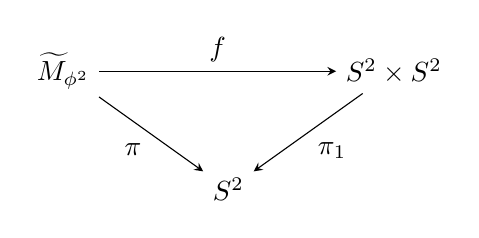
\begin{tikzpicture}[baseline=(current bounding box.center),>=stealth]
  \node (m) at (0,0) {$\widetilde M_{\phi^2}$};
  \node (prod) at (4.2,0) {$S^2\times S^2$};
  \node (base) at (2.1,-1.5) {$S^2$};
  \draw[->] (m) -- node[above] {$f$} (prod);
  \draw[->] (m) -- node[below left] {$\pi$} (base);
  \draw[->] (prod) -- node[below right] {$\pi_1$} (base);
\end{tikzpicture}
\]
其中 $f$ 是微分同胚。如命题~\ref{prop:9-6-4} 的证明所述，\BookRecordIndex{T0279}纤维化
$\pi:\widetilde M_{\phi^2}\to S^2$ 有由生成哈密顿量的两个\BookRecordIndex{T0233}临界点
$[1:0],[0:1]$ 给出的两个自然截面；可以定义 $f$，把它们分别送到平凡丛
$\pi_1:S^2\times S^2\to S^2$ 的对角截面和反对角截面。因此，在
$S^2\times S^2$ 的模型 $\widetilde M_{\phi^2}=S^3\times_{S^1}S^2$ 中，环路
$\{\psi_t\}$ 旋转 $S^2$ 因子：
\[
  t\mathbin{\boldsymbol\cdot}[z_1,z_2;[w_0:w_1]]
  =[z_1,z_2;[w_0:e^{2\pi it}w_1]].
\]
显然，若取
$\widetilde\omega_c=\widetilde\omega+\kappa\pi^*\sigma$，其中
$\widetilde\omega$ 如式~\eqref{eq:9-6-3}，则这个作用保持 $\widetilde\omega_c$。由于生成函数
$H:S^2\to\mathbb R$ 的值落在 $[-1,1]$ 内，对任意 $\lambda>1$ 都可选
$\kappa=\lambda$。于是 $f_*\widetilde\omega_\lambda$（这里用 $f_*$ 表示
$(f^{-1})^*$）与 $\omega_\lambda$ 上同调；只须证明这两个形式同痕。

我们显式应用\BookRecordIndex{T0359}辛膨胀过程来证明这一点。这是一个一般过程：对具有足够多非零 Gromov
不变量的所有辛四维流形，它可以把形变转化为同痕；见 McDuff \srcite{266}。这一过程
最早由 Lalonde 与 McDuff \srcite{258,221,225} 引入，后来又由 Biran
\srcite{38,39} 用于\BookRecordIndex{T0366}辛装填问题。

先同痕 $f$，使 $f_*\widetilde\omega_\lambda=\omega_\lambda$ 在对角线 $\Delta$ 的某个
邻域 $U$ 上成立，再考虑线性道路
\[
  t f_*\widetilde\omega_\lambda+(1-t)\omega_\lambda,
  \qquad 0\le t\le1.
\]
这些形式在 $\pi_1$ 的纤维上非退化。因此，加入拉回 $\pi_1^*\sigma$ 的适当倍数后，
可得到一族（彼此不上同调的）\BookRecordIndex{T0363}辛形式 $\tau_t$，它连接
$\tau_0=\omega_\lambda$ 与 $\tau_1=f_*\widetilde\omega_\lambda$；并且在 $U$ 上有
\[
  \tau_t=c_t\pi_1^*\sigma+\pi_2^*\sigma,
\]
其中 $c_t\ge\lambda$，且当 $t$ 接近 $0,1$ 时等号成立。现在要把形变 $\tau_t$ 转化为
同痕
\[
  \omega_{\lambda,t}
  =\frac1{1+\kappa_t}(\tau_t+\kappa_t\rho_t),
  \qquad t\in[0,1],
\]
它从 $\omega_{\lambda,0}=\omega_\lambda$ 连接到
$\omega_{\lambda,1}=f_*\widetilde\omega_\lambda$。这里形式 $\rho_t$ 支持在 $\Delta$
附近，并表示与 $\Delta$ Poincaré 对偶的类；常数
\[
  \kappa_t:=\frac{c_t-\lambda}{\lambda-1}
\]
选取成使 $[\omega_{\lambda,t}]$ 保持不变。（正是在这里需要 $\lambda>1$。）因此必须
找到 $\rho_t$，使得给 $\tau_t$ 加上它的任意大倍数都不影响非退化性。这些形式之所以
存在，是因为 $\tau_t$ 在 $\Delta$ 上不消失。

细节如下。用 $\pi:L\to S^2$ 表示 Chern 数为 $2$ 的复线丛，并设 $\alpha$ 是相应
$S^1$-丛上的联络 $1$-形式，使
\[
  -d\alpha=2\pi^*\sigma.
\]
若 $r:L\to\mathbb R$ 是纤维中的径向坐标，而
$\beta:[0,1]\to[0,1]$ 是在 $r=0$ 附近等于一的非增\BookRecordIndex{T0188}截断函数，则紧支形式
$-d(\beta(r)\alpha)$ 在每条纤维上的积分为一，在零截面 $L_0$ 上的积分为二。由辛邻域
定理，存在一族光滑嵌入 $g_t:(U,\Delta)\to(L,L_0)$，满足
\[
  (g_t)_*(c_t\pi_1^*\sigma+\pi_2^*\sigma)
  =\frac{c_t+1}{2}\,d\bigl((r^2-1)\alpha\bigr),
  \qquad t\in[0,1].
\]
这里补正外微分的作用对象与系数。
\sourcefootnote{原书右端印作
$\frac{c_t}{2}(d(r^2-1)\alpha)$：其一，括号使 $d$ 只施于标量 $r^2-1$，漏掉
$(r^2-1)d\alpha$ 项；其二，分子还漏了加项 $+1$（等价地系数少了 $1/2$）。事实上，左端在对角线上的限制为
$(c_t+1)\sigma$，而由 $-d\alpha=2\pi^*\sigma$，
$d((r^2-1)\alpha)$ 在零截面上的限制为 $2\pi^*\sigma$，故右端唯一应为
$\frac{c_t+1}{2}d((r^2-1)\alpha)$。}
现在对每个 $t$ 选取支集包含在 $g_t$ 像中的\BookRecordIndex{T0188}截断函数 $\beta_t$，并令
$\rho_t=-d(\beta_t(r)\alpha)$。它们在 $g_t$ 下的拉回具有所需的全部性质。这就完成了
命题~\ref{prop:9-7-2}(ii) 的第二个证明。
\end{proof}

类似论证表明，形式
\[
  \tau_1^k:=(\Psi^{\circ k})_*\tau_1^0,
  \qquad k\ge0,
\]
中任意两个都不同痕，尽管它们全都彼此上同调且形变等价。还可改进这一构造，在如下
八维流形 $\widetilde Y$ 上得到一族形变等价、彼此上同调但不微分同胚的形式：先给
$S^2\times S^2\times\mathbb T^2$ 再乘一个 $S^2$ 因子得到 $Y$，然后沿子流形
\[
  Z:=S^2\times\{w_1\}\times\mathbb T^2\times\{x_1\}
\]
吹起。由于 $Z$ 的余维为 $4$，\personlater{geluomofu}{格罗莫夫}{Gromov}的辛嵌入
定理（见 \srcite{161}，也见 Eliashberg--Mishenko \srcite{102}）说明，对
$j=0,1$，它都能关于 $\tau_1^j+\pi_3^*\sigma$ 辛嵌入到 $Y$ 中。因此，这两个形式在
吹起后给出 $\widetilde Y$ 上的两个\BookRecordIndex{T0363}辛形式 $\widetilde\tau_1^j$；它们在 $Z$ 的吹起
$\widetilde Z$ 上非退化。现在反设存在微分同胚
\[
  f:(\widetilde Y,\widetilde\tau_1^0)
  \longrightarrow(\widetilde Y,\widetilde\tau_1^1).
\]
考察例外除子类 $E$ 中曲线的\BookRecordIndex{T0246}模空间，可以证明（粗略地说）：由
$\pi_2\circ f$ 给出的、从 $\widetilde Z$ 到 $\widetilde Y$ 中第二个 $S^2$ 因子的映射
必为零伦的。另一方面，$(\widetilde Y,\widetilde\tau_1^j)$ 的子流形
\[
  W=S^2\times S^2\times\mathbb T^2\times\{x_2\}
\]
包含一参数 $A$-全纯曲线族，它们绕第二个 $S^2$ 因子扭转 $j$ 次。由于 $Z$ 可以同伦
到 $W$ 中，把这一事实与从 $E$-曲线所得的信息比较，就会导出矛盾。

这里有一个值得注意的解析问题。由于 $\widetilde\tau_1^j(E)$ 很小，类
$A\in H_2(\widetilde Y)$ 不再不\BookRecordIndex{T0213}可分解，\BookRecordIndex{T0246}模空间 $\mathcal M(A;J)$ 具有非空边界。对每个
$J$，我们关心的是一参数 $A$-曲线族的性质，所以必须考虑
$\mathcal M(A;J_t)$（$t\in[0,1]$）中元素的二参数族。因此，这些族一般不紧；我们不能
再通过扰动道路 $\{J_t\}$ 来避免碰到边界。不过，可以分析极限\BookRecordIndex{T0340}稳定映射，并证明它们不
影响不变量 $\chi$。根本原因是，投影
$\pi_2:\widetilde Y\to S^2$ 在极限\BookRecordIndex{T0340}稳定映射的每个分支上次数都为零。若一条 $A$-曲线
能分解为一条 $(A-B)$-曲线与一条 $B$-曲线之和，则这个论证会失效；这里 $B$ 表示第二个
球面的类。这种情形只在 $\lambda>1$ 时可能发生，而此时我们知道论证确实失效。更多
细节见 \srcite{254}。
